\chapter{Rangkuman Langkah-Langkah Pembuatan}

\section{Langkah-Langkah Pembuatan Aplikasi Akademik Sederhana APEX}

\begin{enumerate}


\item[1]Pergi ke Website Oracle APEX, https://apex.oracle.com, lalu klik Sign In.

\begin{figure}[!htbp]
    \begin{center}
    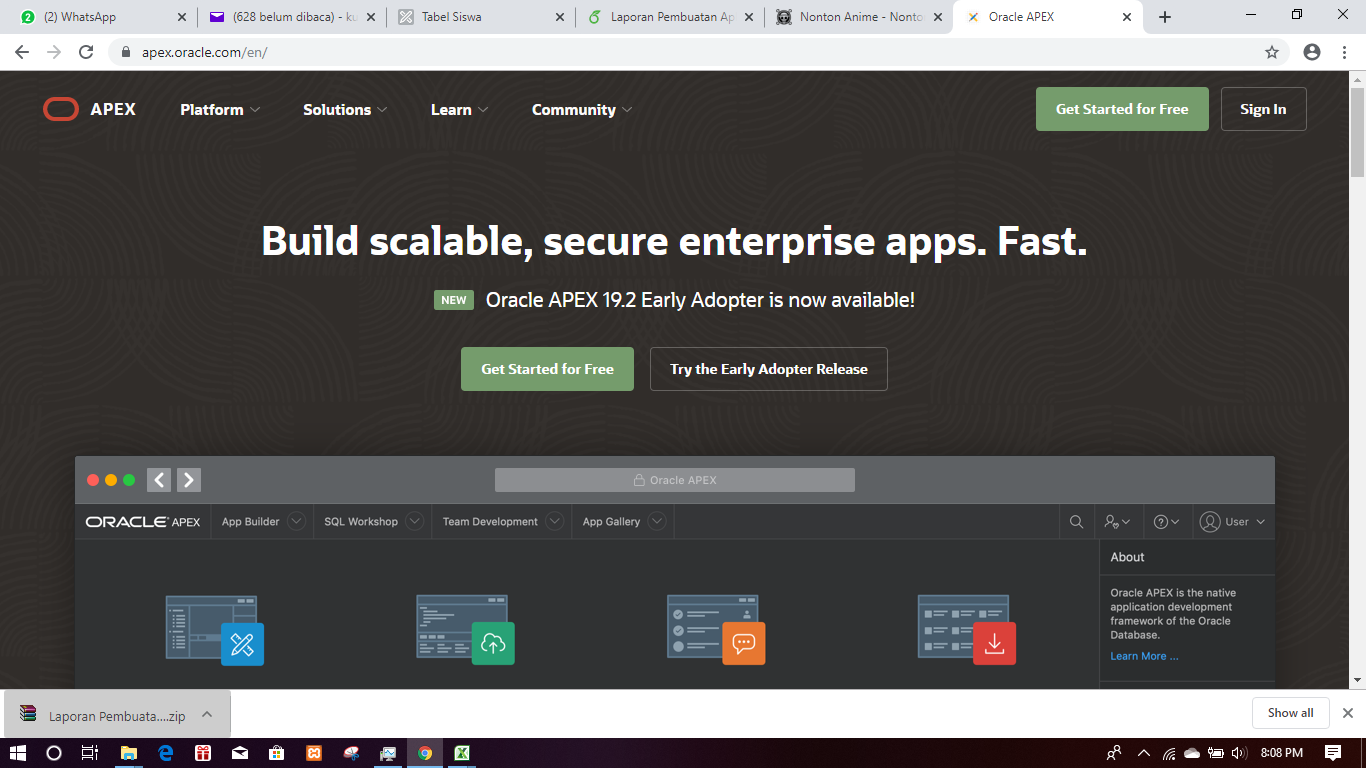
\includegraphics[scale=0.2]{figures/01.png}
    \end{center}
    \end{figure}

\par
Pertama kita harus memiliki Akun Oracle Apex Online, apabila tidak memiliki kita dapat melakukan Register.

\item[2]Kemudian Isi Workspace, Email dan Password.

\begin{figure}[!htbp]
    \begin{center}
    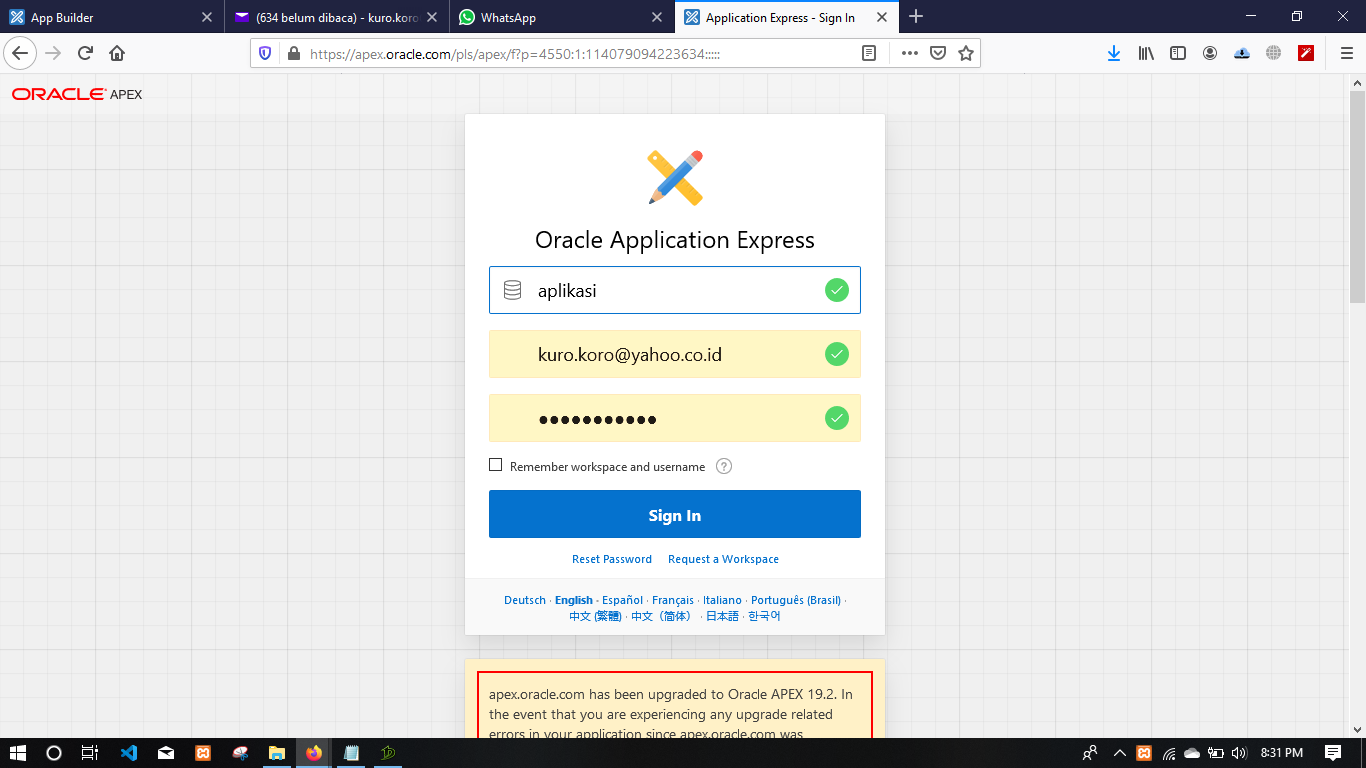
\includegraphics[scale=0.2]{figures/31.png}
    \end{center}   
    \end{figure}

\par
Setelah kita klik Sign in, disana kita harus memiliki Workspace serta Email dan Password yang sudah kalian buat.

\item[3]Kemudian Klik APP BUILDER, Setelah itu Klik Create.

\begin{figure}[!htbp]
    \begin{center}
    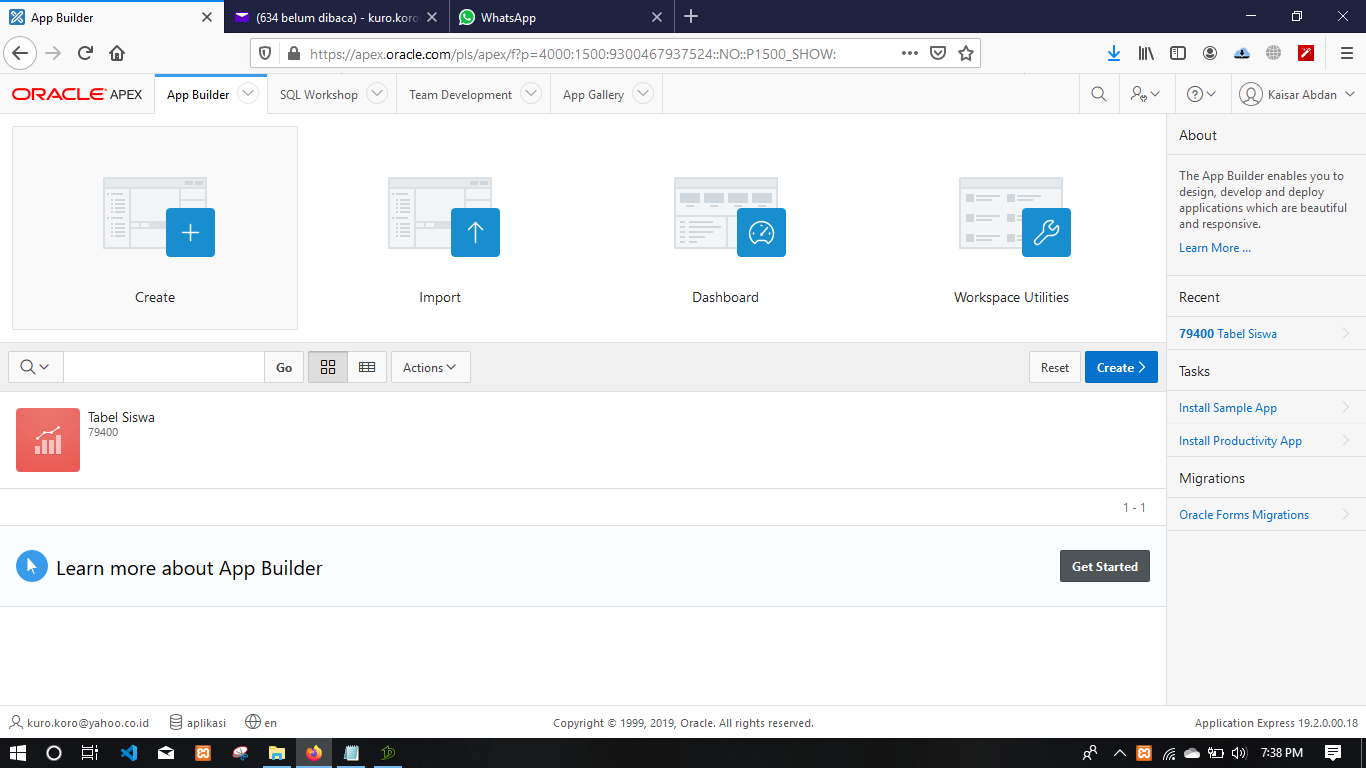
\includegraphics[scale=0.2]{figures/02.png}
    \end{center}   
    \end{figure}

\par
Setelah login kita klik APP BUILDER, Setelah itu Klik Create.

\item[4]Kemudian Klik From a File.

\begin{figure}[!htbp]
    \begin{center}
    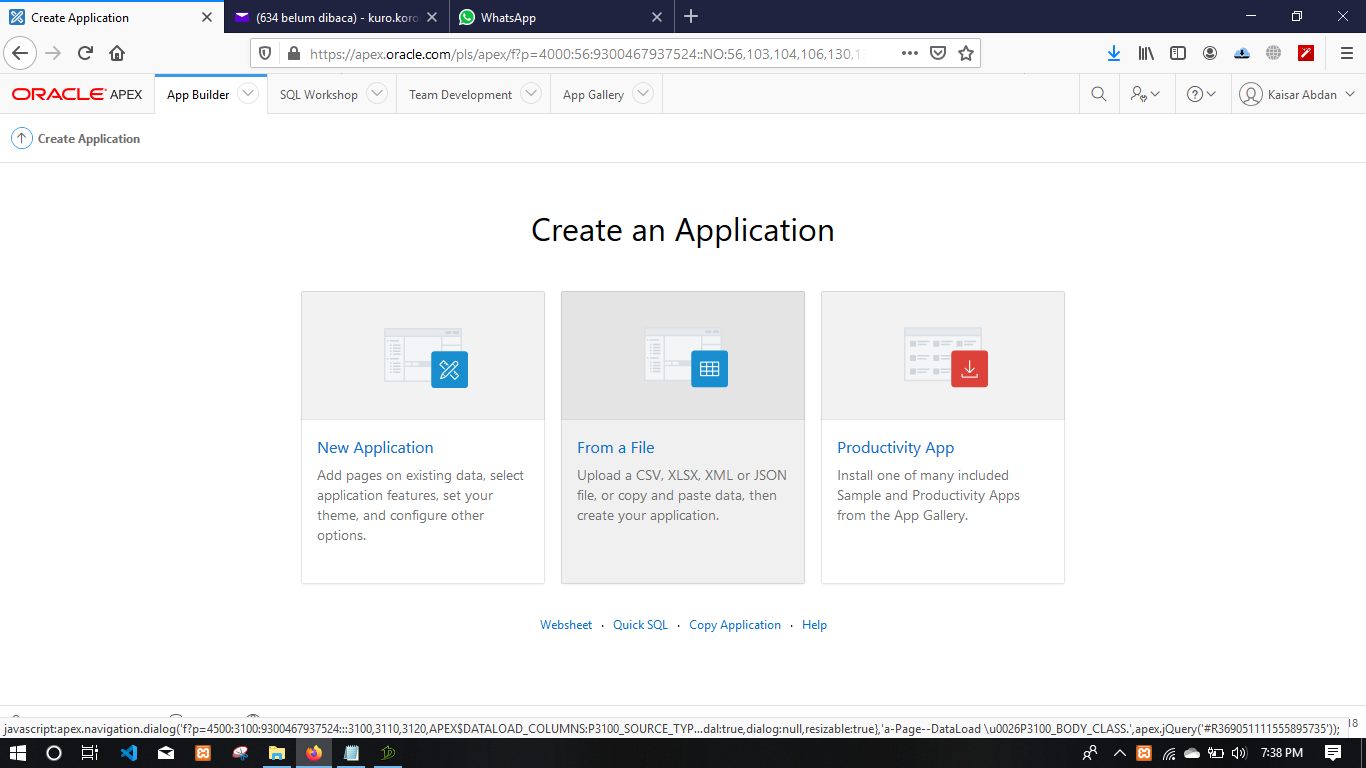
\includegraphics[scale=0.2]{figures/03.png}
    \end{center}   
    \end{figure}

\par
Kemudian Disini kita Bertujuan Untuk Mengambil File dari Folder kita.

\newpage
\item[5]Kemudian Drag And Drop.

\begin{figure}[!htbp]
    \begin{center}
    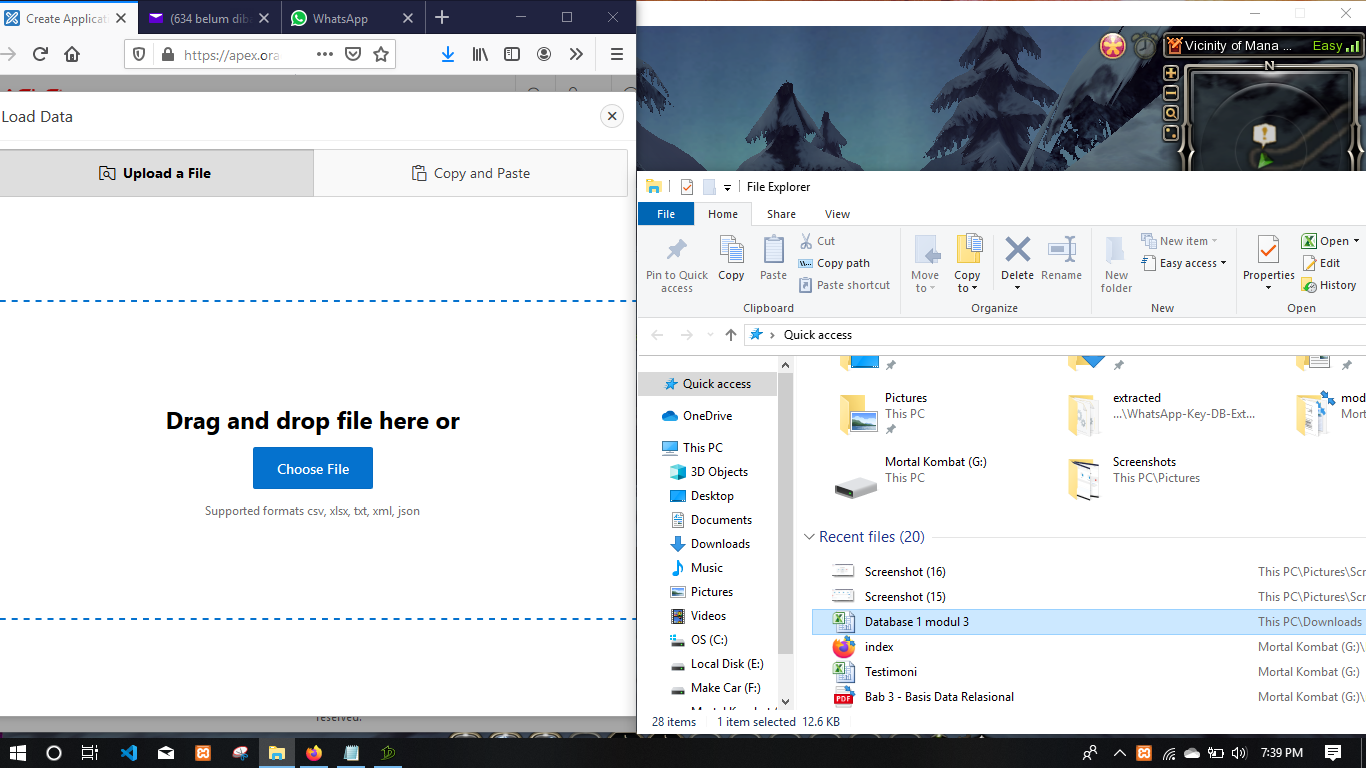
\includegraphics[scale=0.2]{figures/04.png}
    \end{center}   
    \end{figure}

\par
Drag And Drop ini ya digunakan untuk mengambil file dari folder kita yaitu folder yang sudah kita buat di excel.

\item[6]Kemudian Kita Melakukan Pengisian Semua.

\begin{figure}[!htbp]
    \begin{center}
    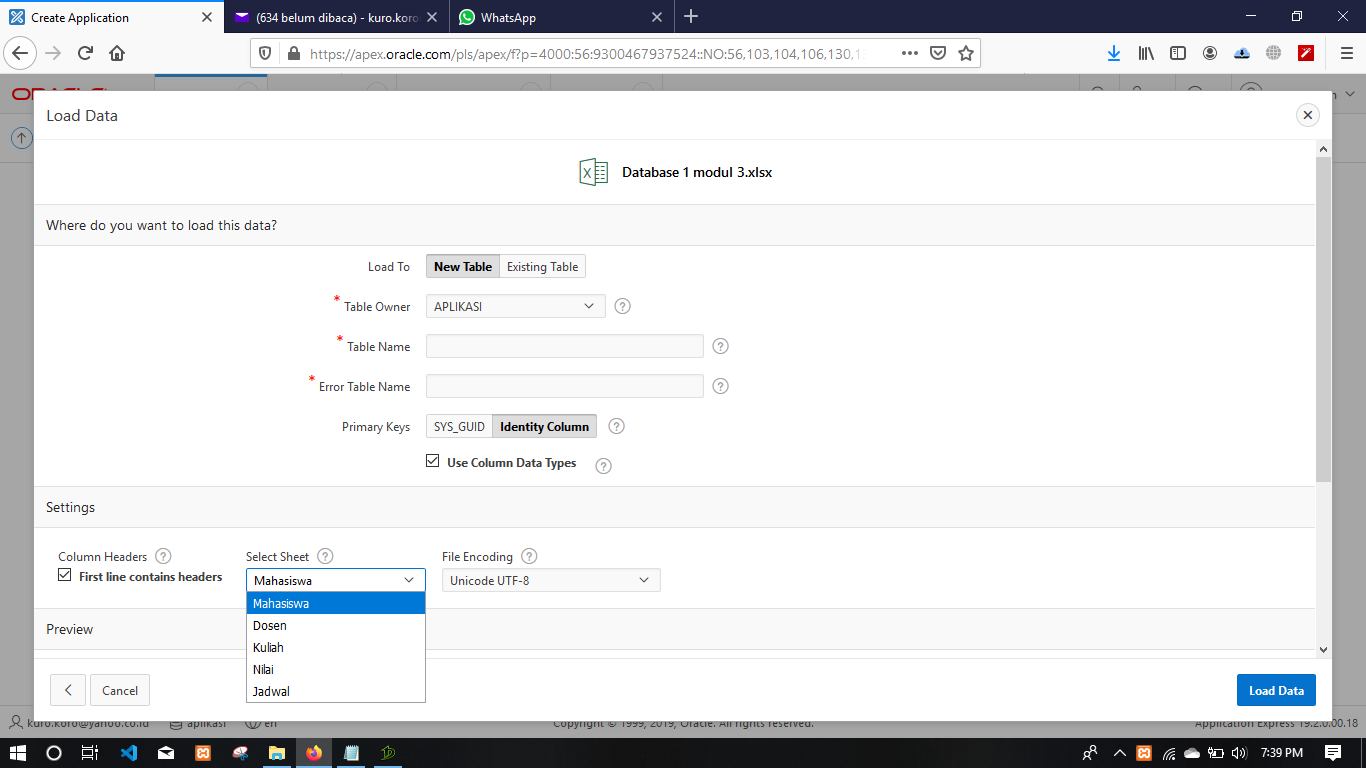
\includegraphics[scale=0.2]{figures/05.png}
    \end{center}   
    \end{figure}

\par
Pengisian Seperti Table Name Sesuaikan Saja Seperti Nama Sheetnya dan Melakukan Pemilihan Select Sheet, dari Mahasiswa, Dosen, Kuliah, Nilai, dan Jadwal.

\newpage
\item[7]Kemudian Klik SQL Workshop

\begin{figure}[!htbp]
    \begin{center}
    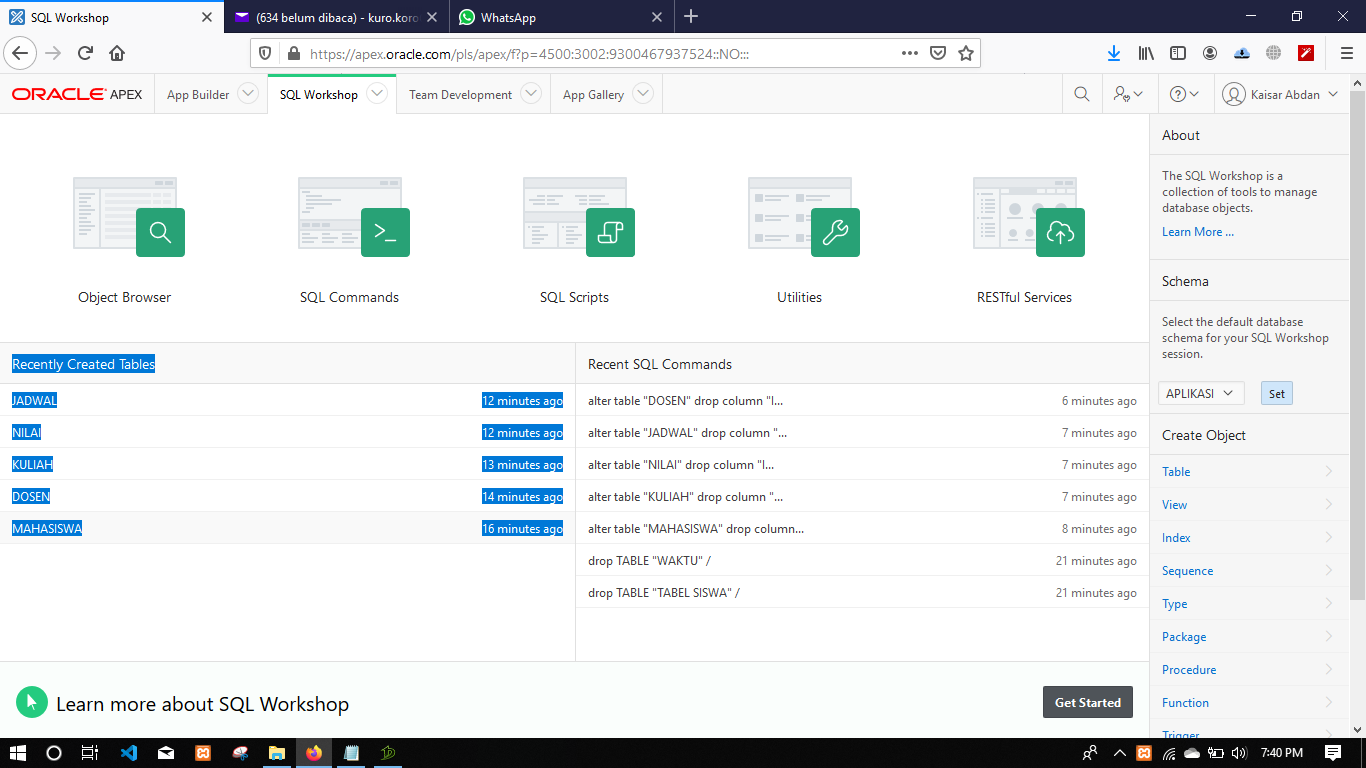
\includegraphics[scale=0.2]{figures/06.png}
    \end{center}   
    \end{figure}
    
\par
Kemudian setelah kita melakukan pengisian semua, langkah selanjutnya kita klik SQL Workshop untuk mengecek Recent Create Tablenya.

\item[8]Kemudian Klik Mahasiswa Pada Recent Create Table di gambar sebelumnya

\begin{figure}[!htbp]
    \begin{center}
    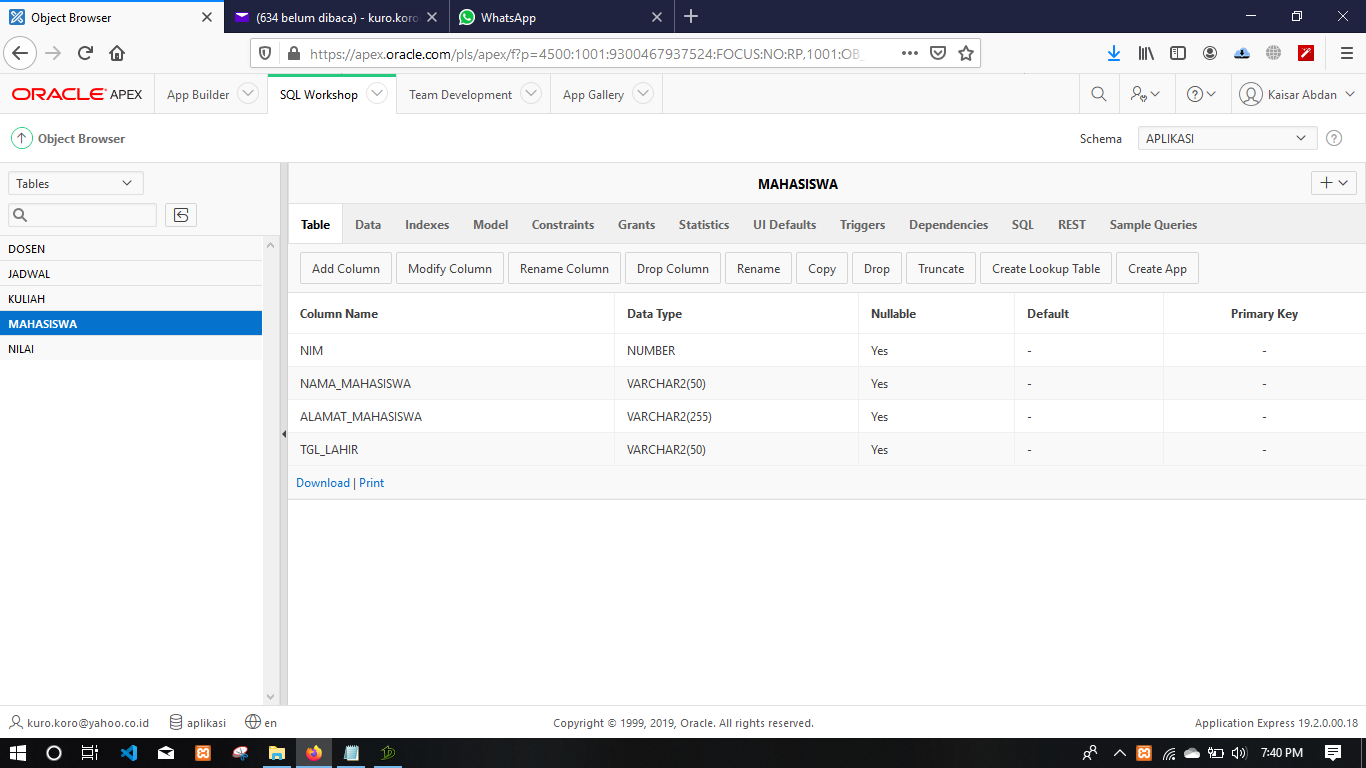
\includegraphics[scale=0.2]{figures/07.png}
    \end{center}   
    \end{figure}
    
\par
Kemudian setelah itu kita bisa mengecek DataType pada Mahasiswa, kemudian klik Drop Column untuk menghapus ID pada Coloum Name.

\newpage
\item[9]Ini Tampilan Saat mau Menghapus ID.

\begin{figure}[!htbp]
    \begin{center}
    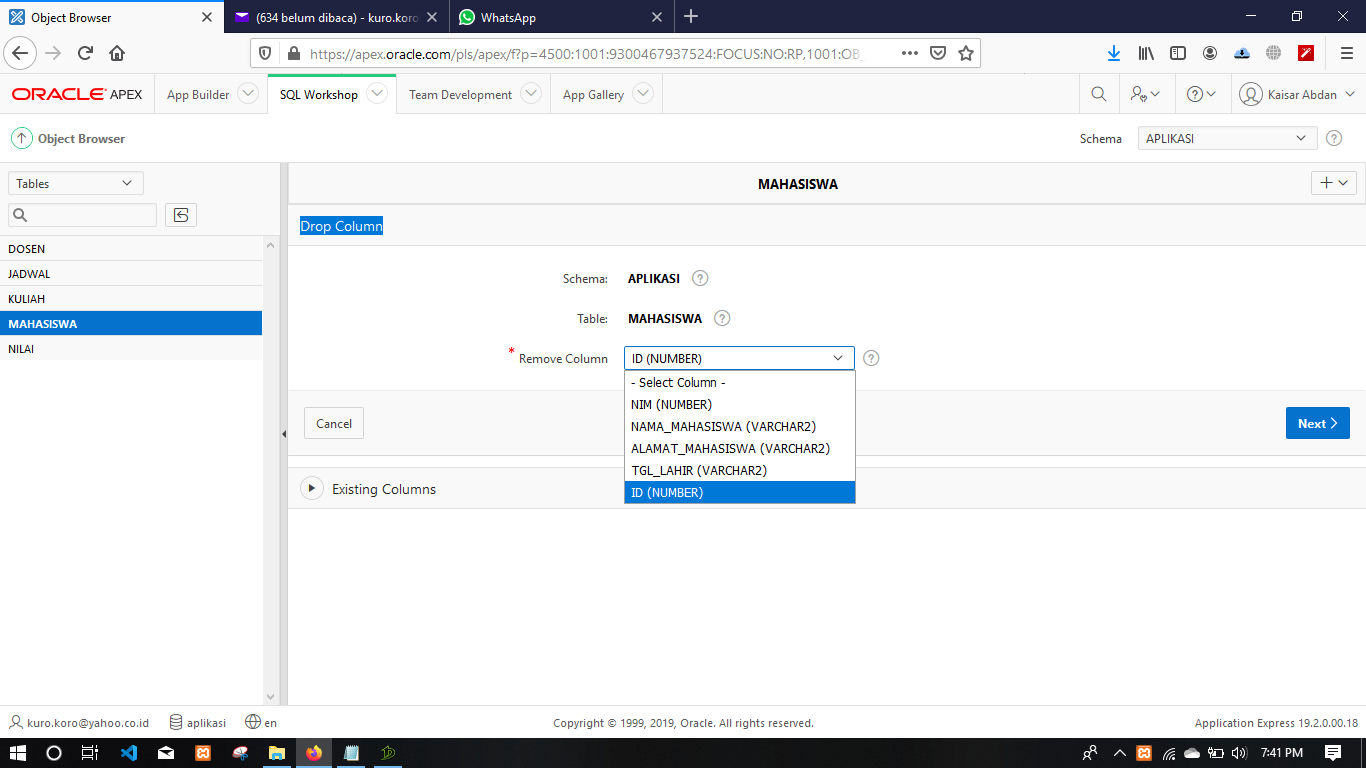
\includegraphics[scale=0.2]{figures/09.png}
    \end{center}   
    \end{figure}
    
\par
Disini kita bertujuan untuk menghapus ID.

\item[10]Setelah itu Kita Klik Constraints

\begin{figure}[!htbp]
    \begin{center}
    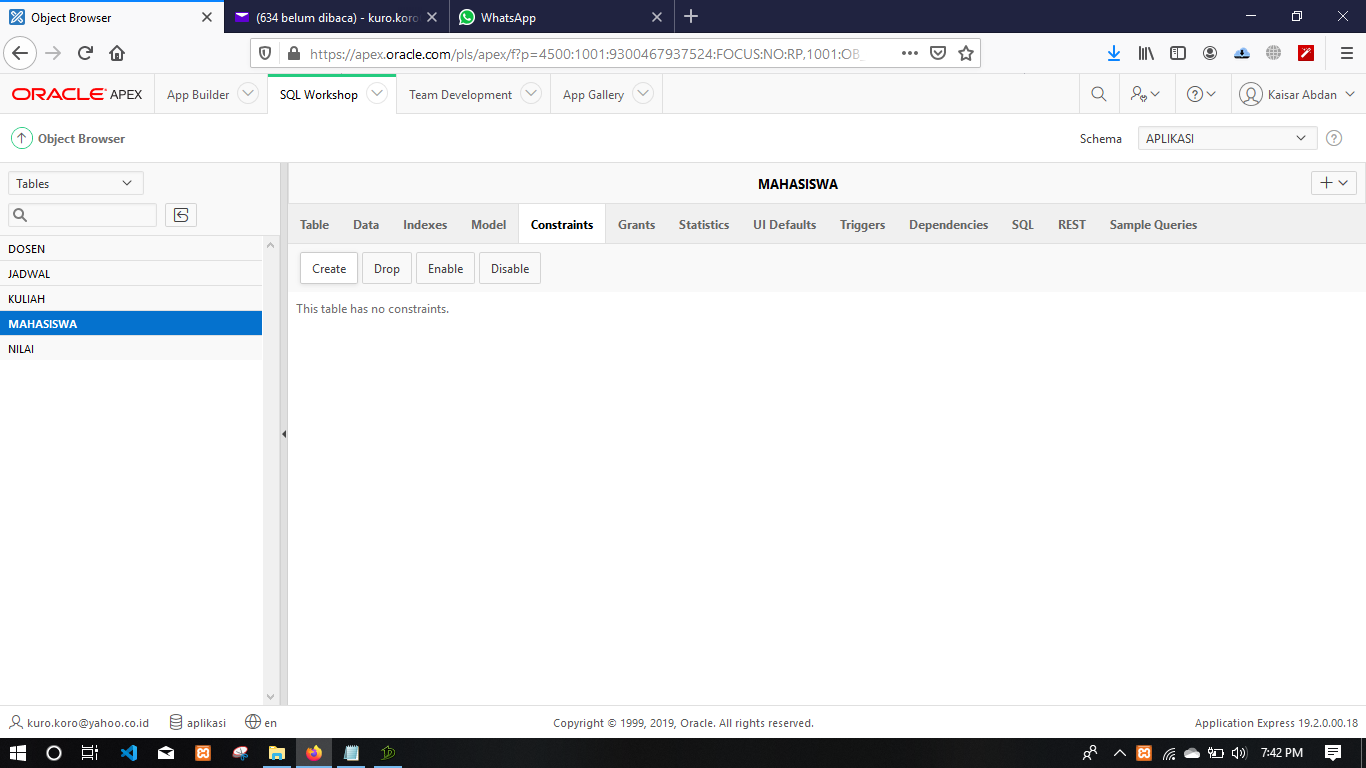
\includegraphics[scale=0.2]{figures/11.png}
    \end{center}   
    \end{figure}
    
\par
Setelah Klik Constraints kita Klik Create.

\newpage
\item[11]Ini Tampilan Setelah kita Klik Create.

\begin{figure}[!htbp]
    \begin{center}
    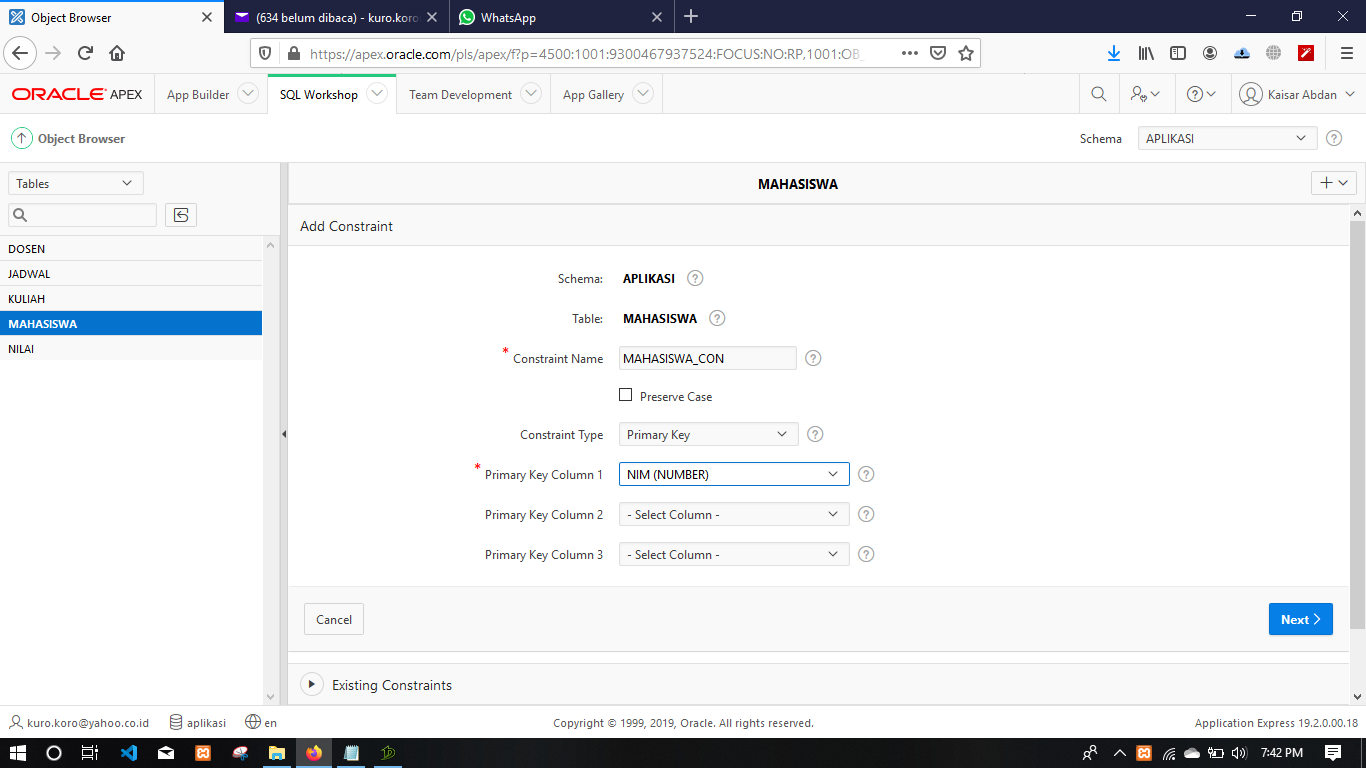
\includegraphics[scale=0.2]{figures/12.png}
    \end{center}   
    \end{figure}
    
\par
Tampilannya Seperti berikut, Disana Kita Bisa Melihat Constraints Name Dan Constraint Type. Constraint Type ada Beberapa pilihan, tetapi kita pilih Primary Key, Primary Key ini digunakan Untuk yang hanya memiliki 1 Primary. Setelah memilih Primary Key Kemudian kita isi NIM sebagai Primary Key. Kemudian kita ke Table DOSEN lakukan langkah yang sama, bedanya Primary key kita pilih NIK. Setelah itu kita ke Table KULIAH lakukan langkah yang sama, bedanya Primary key kita pilih KODE. Kita lakukan Perintah ini hanya Kepada Table DOSEN, MAHASISWA Dan KULIAH.

\item[12]Setelah itu Kita Klik Finish

\begin{figure}[!htbp]
    \begin{center}
    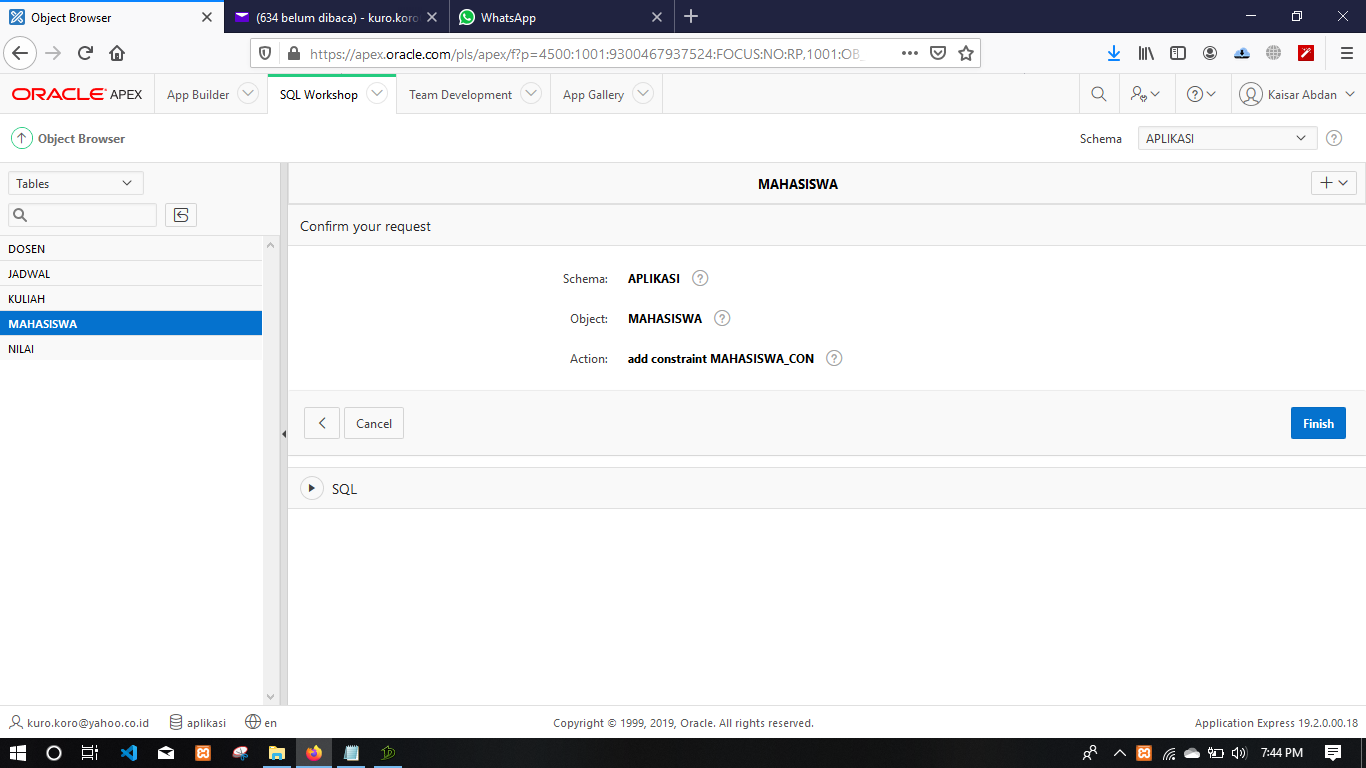
\includegraphics[scale=0.2]{figures/15.png}
    \end{center}   
    \end{figure}
    
\par
Setelah klik Finish, berarti sudah membuat primary key yang baru pada MAHASISWA , DOSEN Dan KULIAH.

\newpage
\item[13]Setelah itu Kita Klik NILAI

\begin{figure}[!htbp]
    \begin{center}
    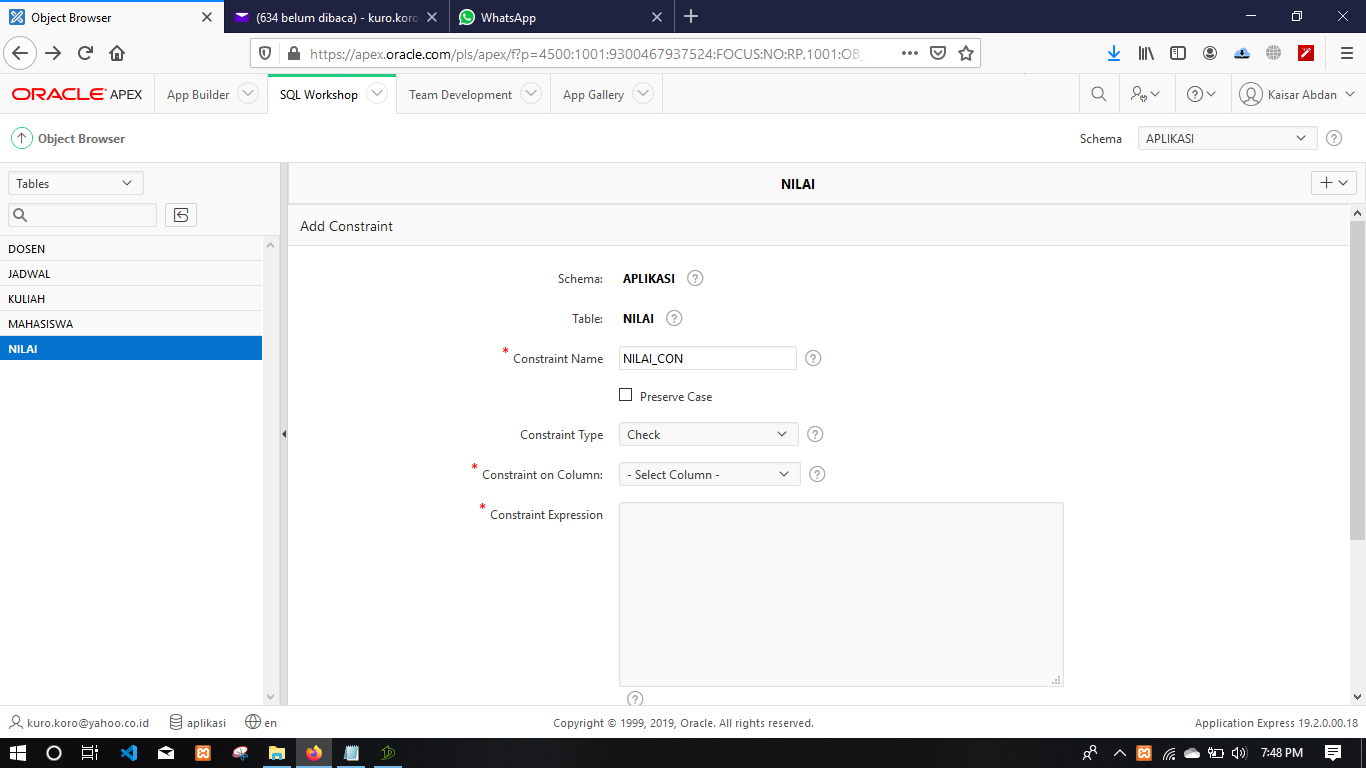
\includegraphics[scale=0.2]{figures/17.png}
    \end{center}   
    \end{figure}
    
\par
Setelah klik NILAI, kita pilih Constraint Type Foreign Key, Kemudian kita Pisahkan Primary Key dengan Foreign Key, Primary Key Seperti NIM Pindahkan Ke Kanan, Kemudian kita cari Table yang memiliki Primary Key NIM.

\item[14]Ini Tampilan Setelah Melakukan Pemilihan Dan Pengisian pada Table NILAI.

\begin{figure}[!htbp]
    \begin{center}
    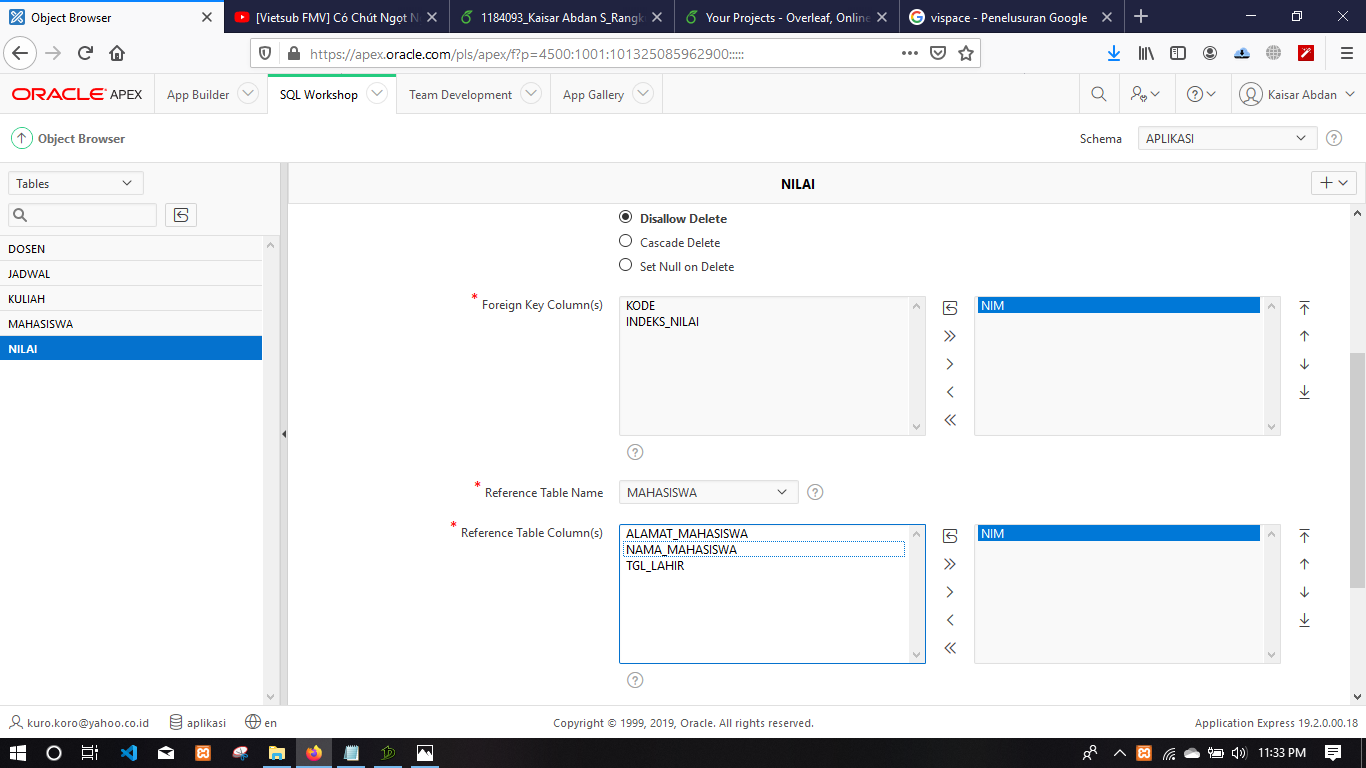
\includegraphics[scale=0.2]{figures/18.png}
    \end{center}   
    \end{figure}
    
\par
Ini Hasil Pengisian kita dapat lakukan ke Table NILAI kita melakukan Relasi NIM dan KODE, yang digambar kita Relasikan NIM maka Relasinya dengan Table MAHASISWA yang ada Primary Key NIM, Setelah merelasikan itu, kita merelasikan lagi yaitu bagian KODE dengan table KULIAH yang ada Primary Key KODE.

\newpage
\item[15]Ini Tampilan Setelah Melakukan Pemilihan Dan Pengisian pada Table JADWAL.

\begin{figure}[!htbp]
    \begin{center}
    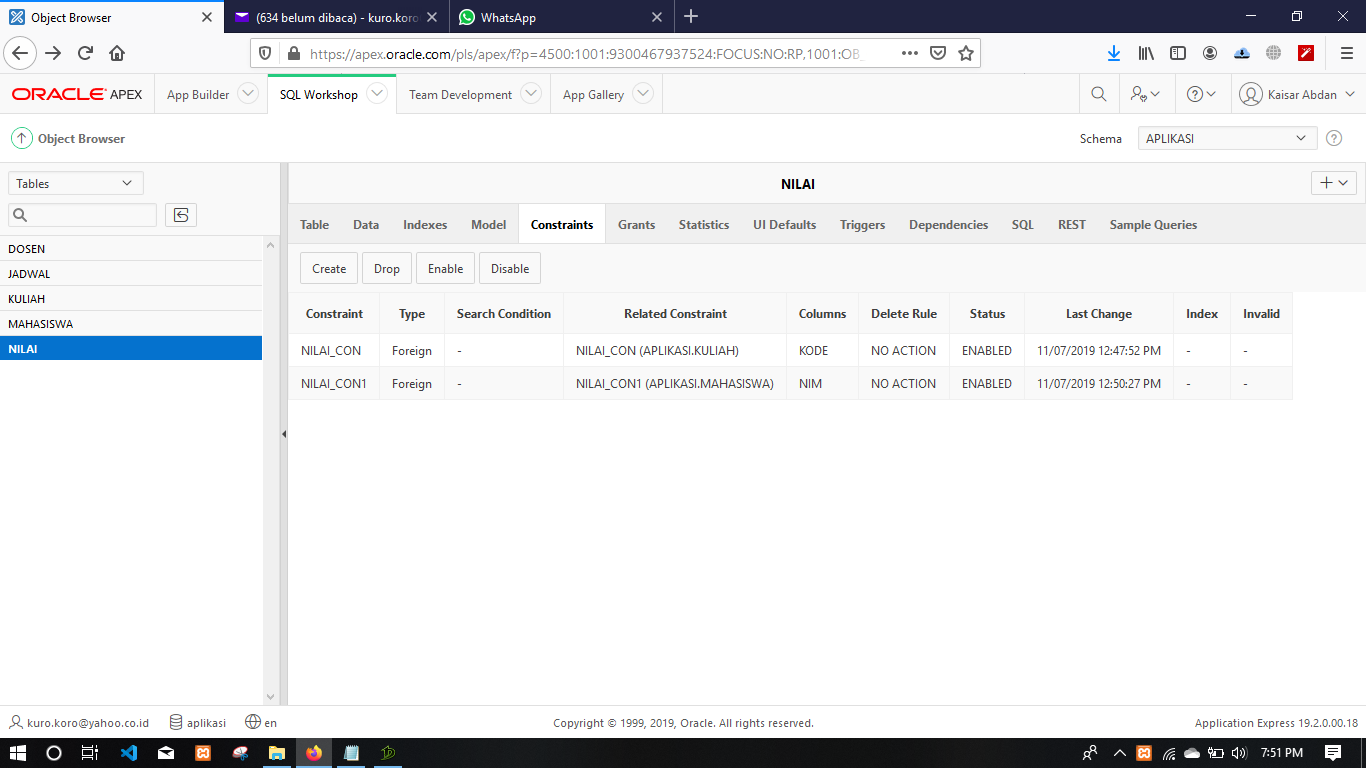
\includegraphics[scale=0.2]{figures/19.png}
    \end{center}   
    \end{figure}
    
\par
Ini Hasil Pengisian kita dapat lakukan ke Table JADWAL kita melakukan Relasi KODE dan NIK, yang digambar kita Relasikan KODE maka Relasinya dengan Table KULIAH yang ada Primary Key KODE, Setelah merelasikan itu, kita merelasikan lagi yaitu bagian NIK dengan Table DOSEN yang ada Primary Key KODE.

\item[16]Setelah itu Kita Klik APP BUILDER, Kemudian New Application

\begin{figure}[!htbp]
    \begin{center}
    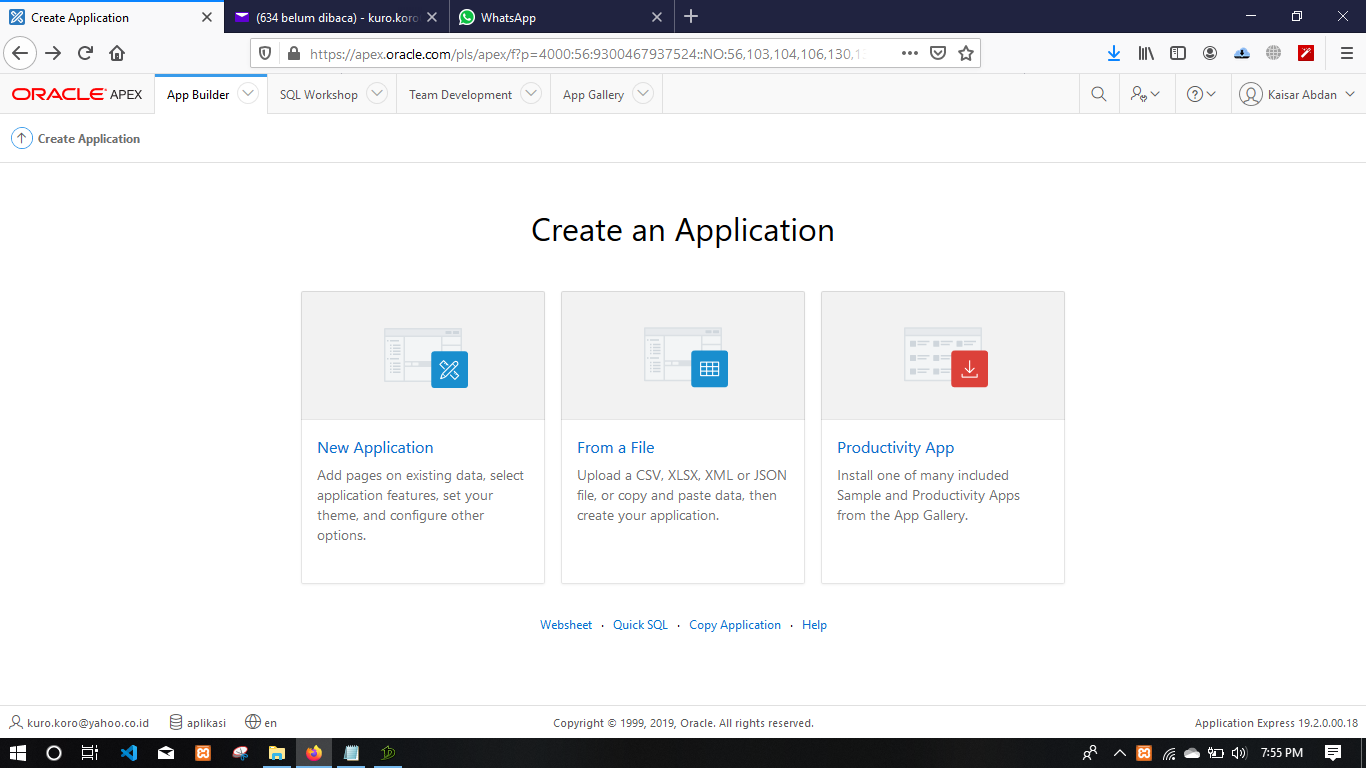
\includegraphics[scale=0.2]{figures/20.png}
    \end{center}   
    \end{figure}
    
\par
Disini kita akan memulai membuat aplikasi

\newpage
\item[17]Tampilan dalam Create a Application

\begin{figure}[!htbp]
    \begin{center}
    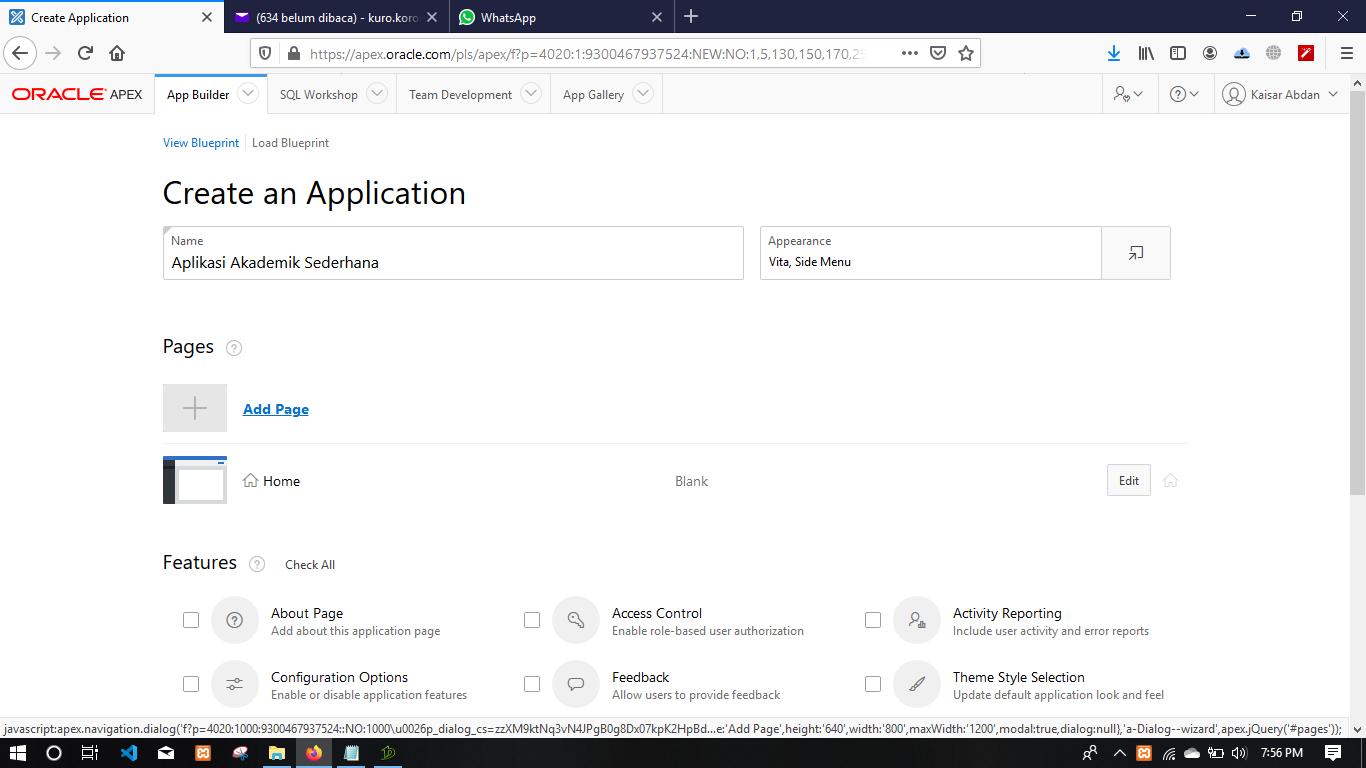
\includegraphics[scale=0.2]{figures/21.png}
    \end{center}   
    \end{figure}
    
\par
Disini kita Mengisi Nama Aplikasinya Dan Menambah Page-Pagenya

\item[18]Ini tampilan Add Page

\begin{figure}[!htbp]
    \begin{center}
    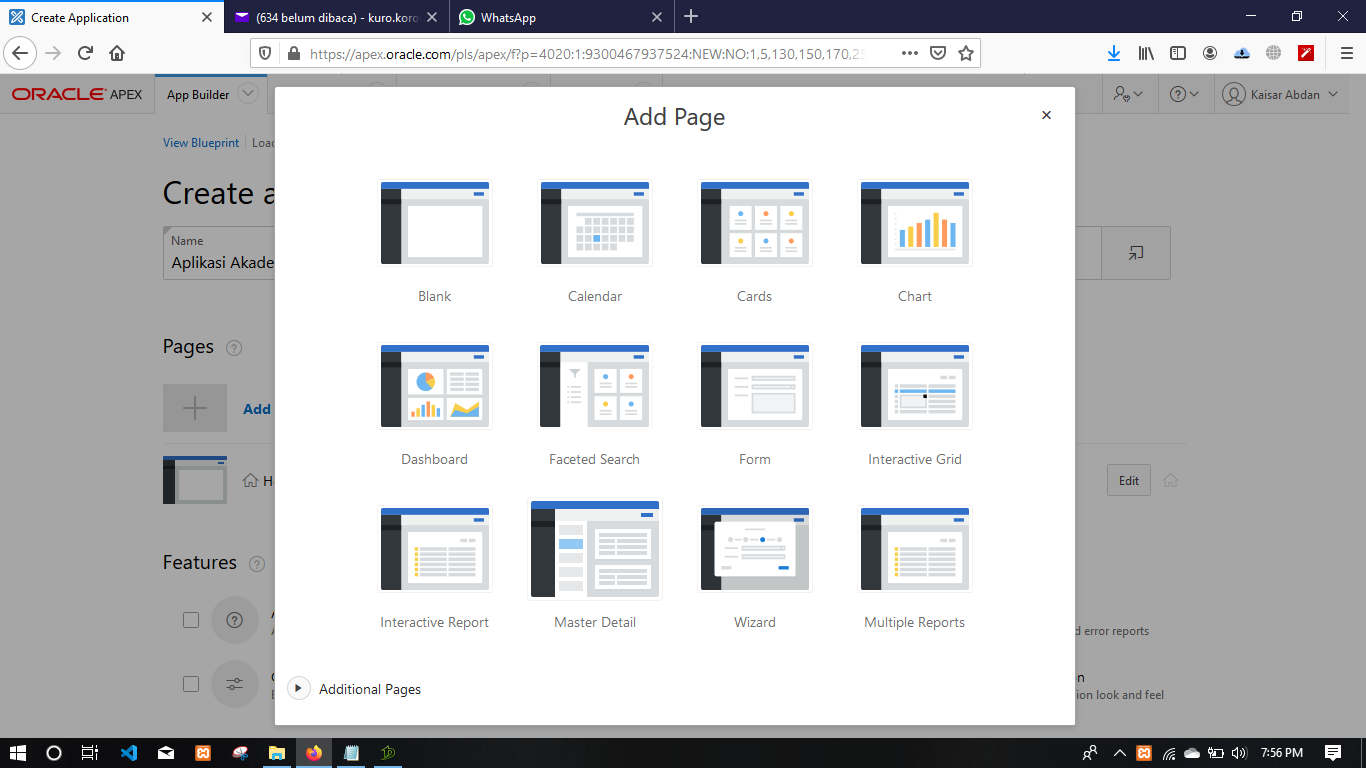
\includegraphics[scale=0.2]{figures/22.png}
    \end{center}   
    \end{figure}
    
\par
Disini kita dapat Memilih Master Detail Untuk Table DOSEN, MAHASISWA Dan KULIAH, Dan Interactive Report digunakan untuk Table JADWAL dan NILAI.

\newpage
\item[19]Ini Tampilan Add Master Detail Page

\begin{figure}[!htbp]
    \begin{center}
    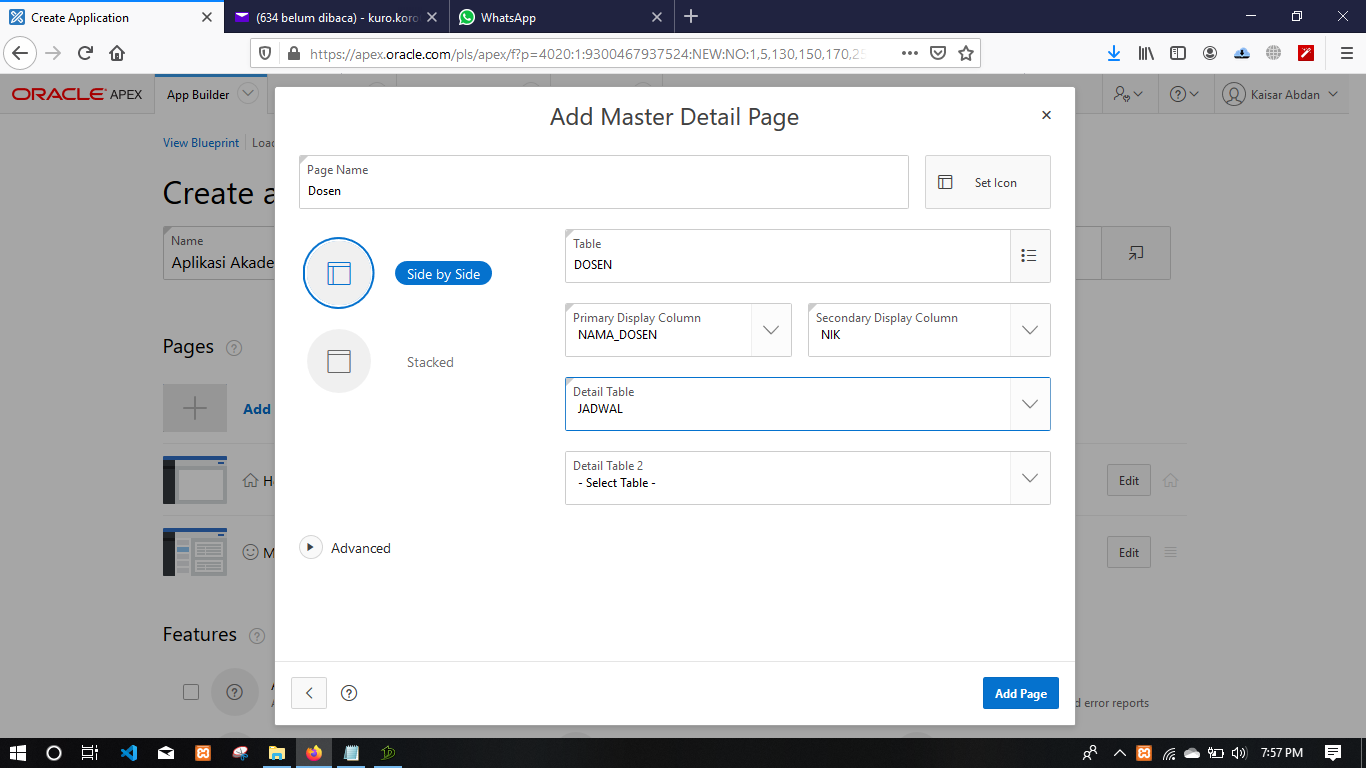
\includegraphics[scale=0.2]{figures/23.png}
    \end{center}   
    \end{figure}
    
\par
Kita Isi Sesuai Dengan Gambar Berikut.

\item[20]Ini Tampilan Add Report Page

\begin{figure}[!htbp]
    \begin{center}
    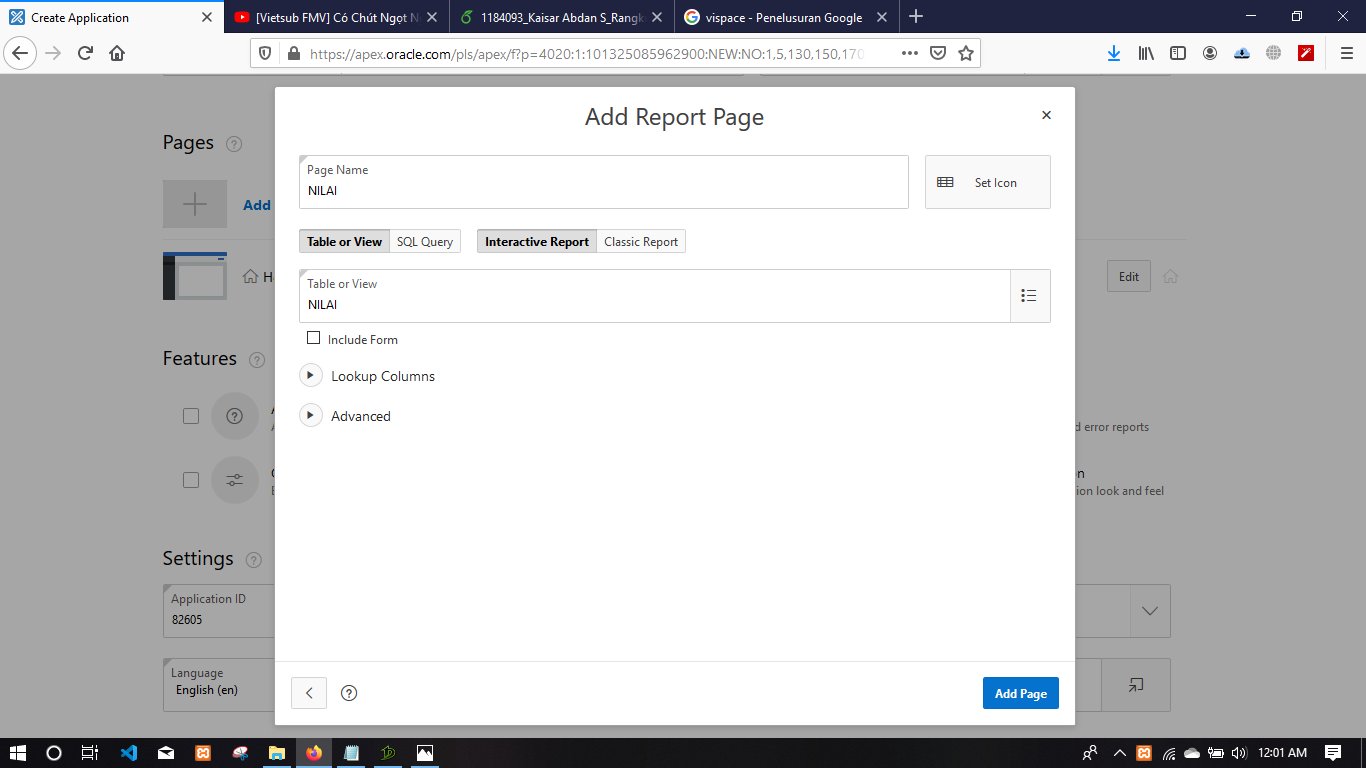
\includegraphics[scale=0.2]{figures/32.png}
    \end{center}   
    \end{figure}
    
\par
Kita Isi Sesuai Dengan Gambar Berikut.

\newpage
\item[21]Ini Tampilan Add Dashboard Page

\begin{figure}[!htbp]
    \begin{center}
    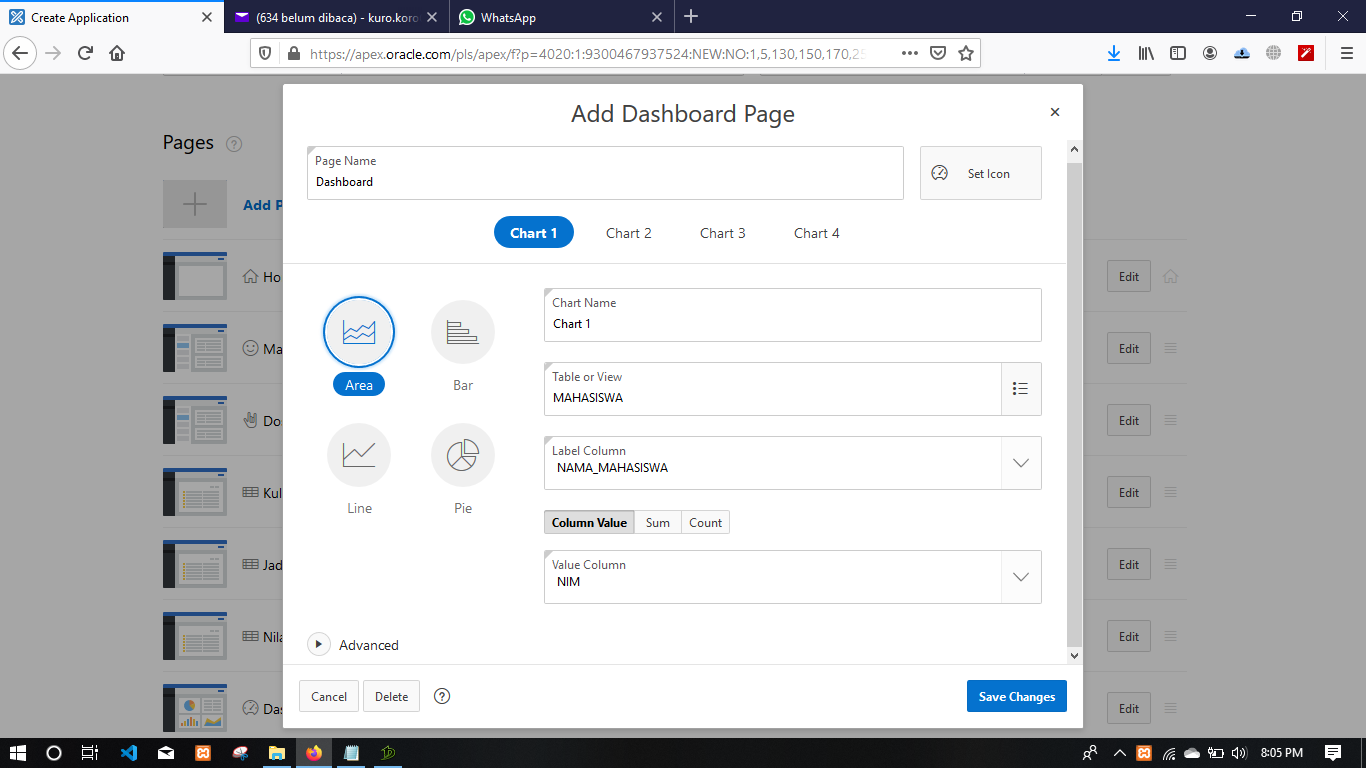
\includegraphics[scale=0.2]{figures/24.png}
    \end{center}   
    \end{figure}
    
\par
Kita Isi Sesuai Dengan Gambar Berikut.

\item[22]Ini Tampilan Add Dashboard Page

\begin{figure}[!htbp]
    \begin{center}
    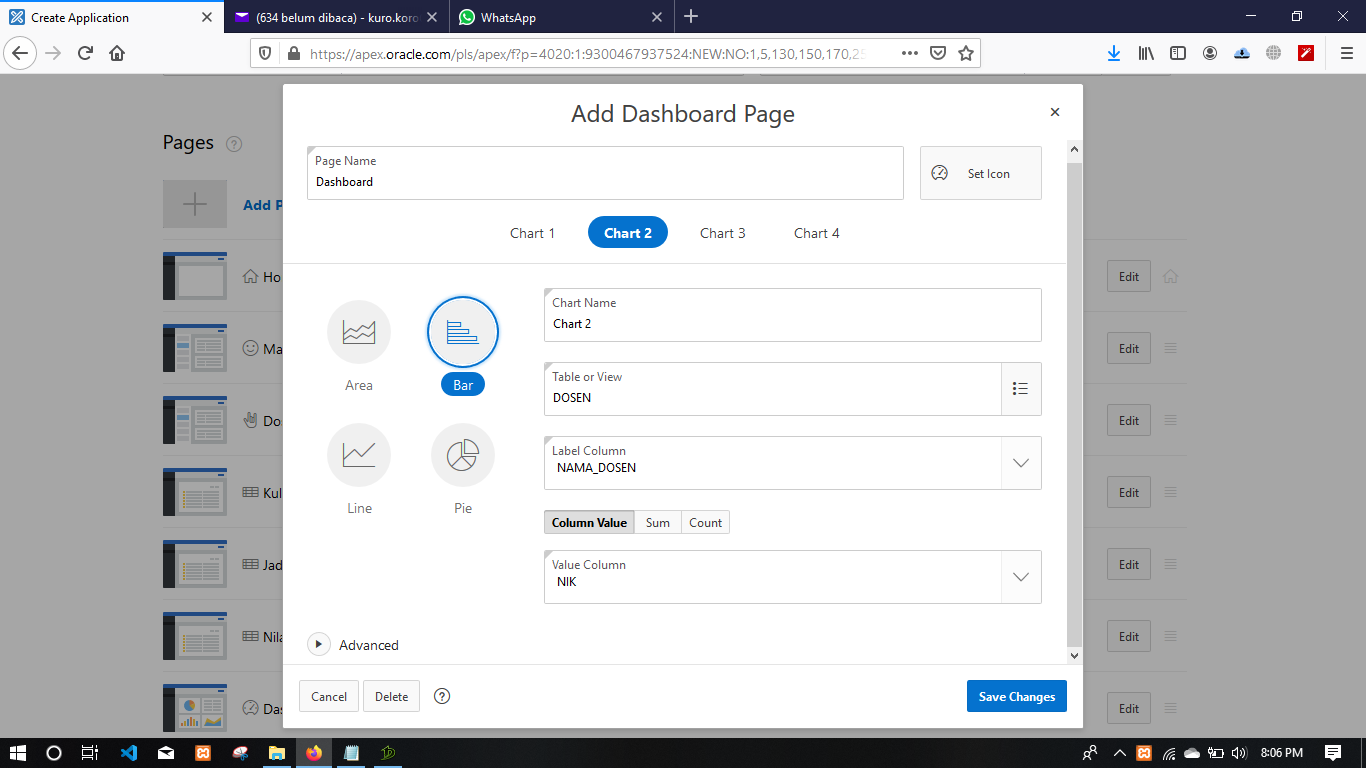
\includegraphics[scale=0.2]{figures/25.png}
    \end{center}   
    \end{figure}
    
\par
Kita Isi Sesuai Dengan Gambar Berikut.

\newpage
\item[23]Ini Tampilan Add Dashboard Page

\begin{figure}[!htbp]
    \begin{center}
    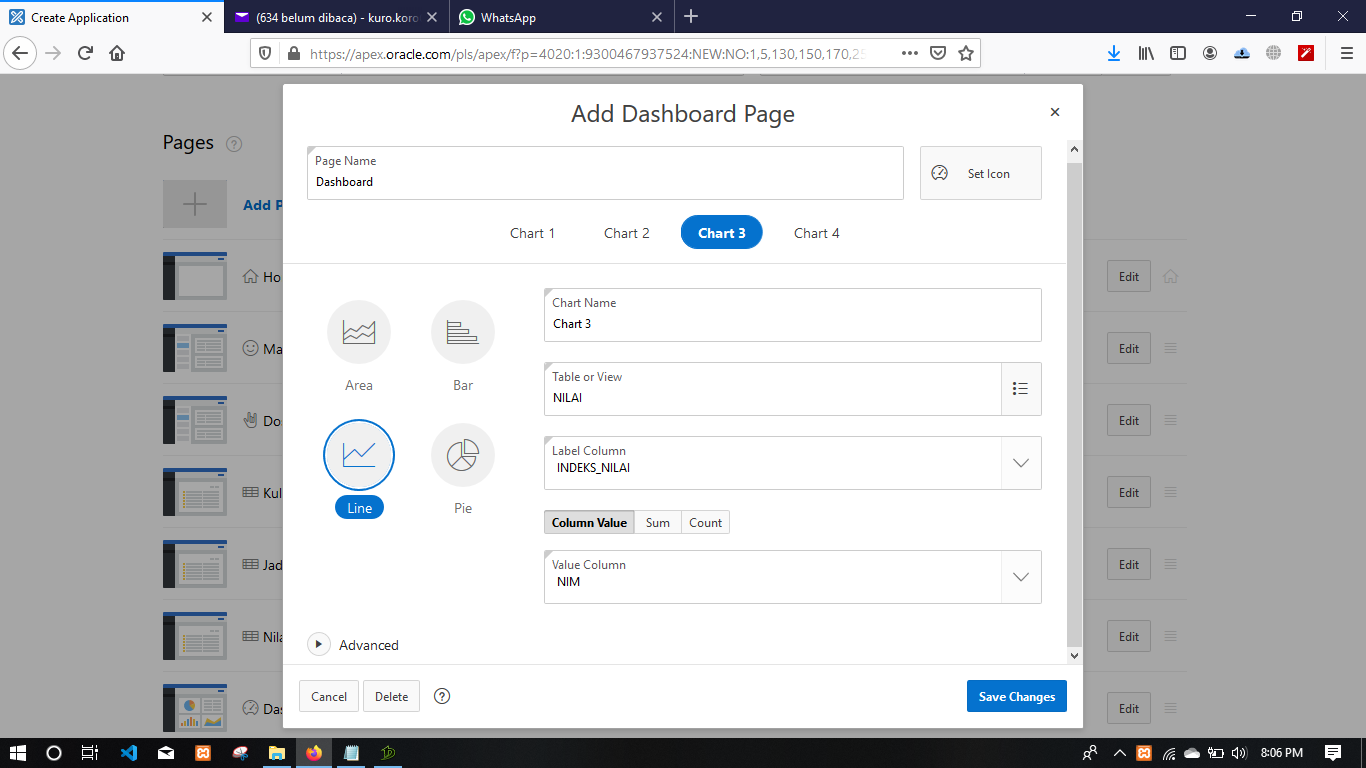
\includegraphics[scale=0.2]{figures/26.png}
    \end{center}   
    \end{figure}
    
\par
Kita Isi Sesuai Dengan Gambar Berikut.

\item[24]Ini Tampilan Add Dashboard Page

\begin{figure}[!htbp]
    \begin{center}
    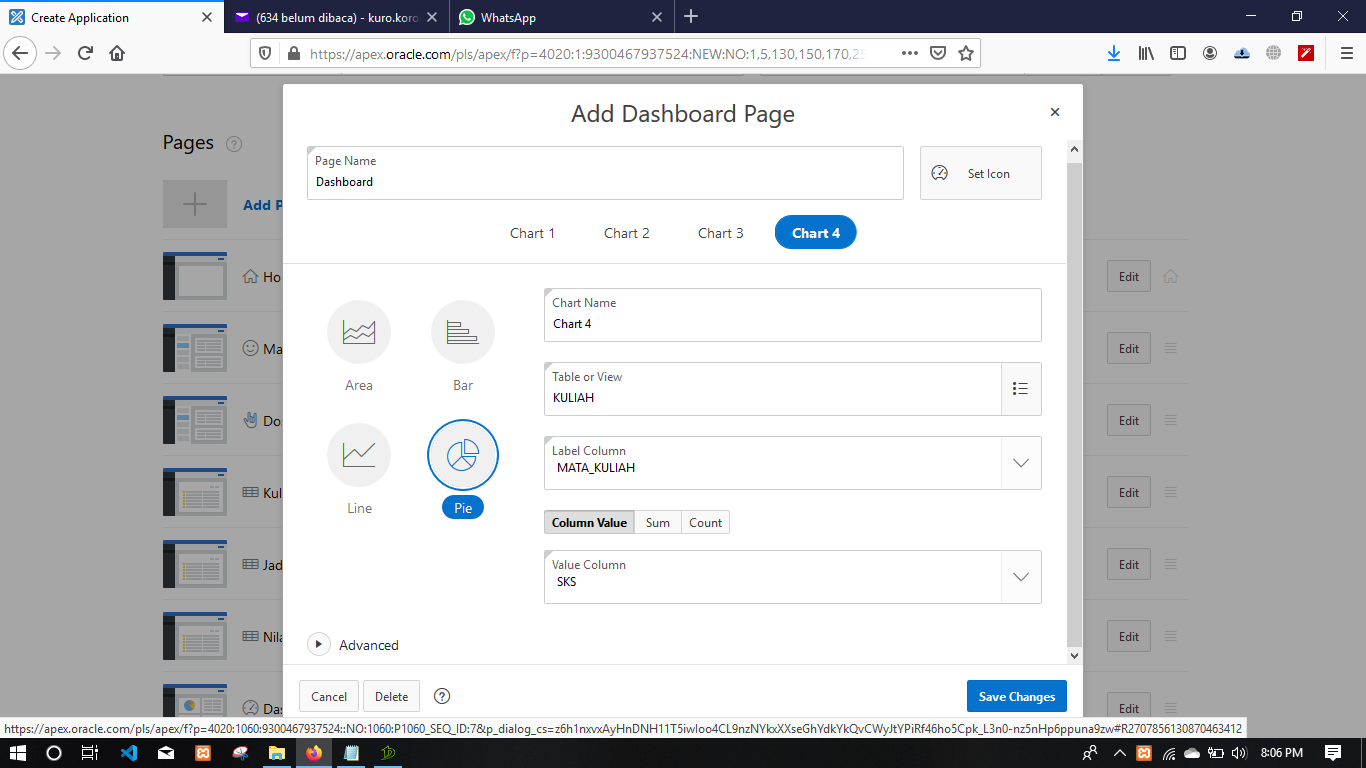
\includegraphics[scale=0.2]{figures/27.png}
    \end{center}   
    \end{figure}
    
\par
Kita Isi Sesuai Dengan Gambar Berikut.

\newpage
\item[25]Ini Tampilan Setelah Mengisi Page-Pagenya

\begin{figure}[!htbp]
    \begin{center}
    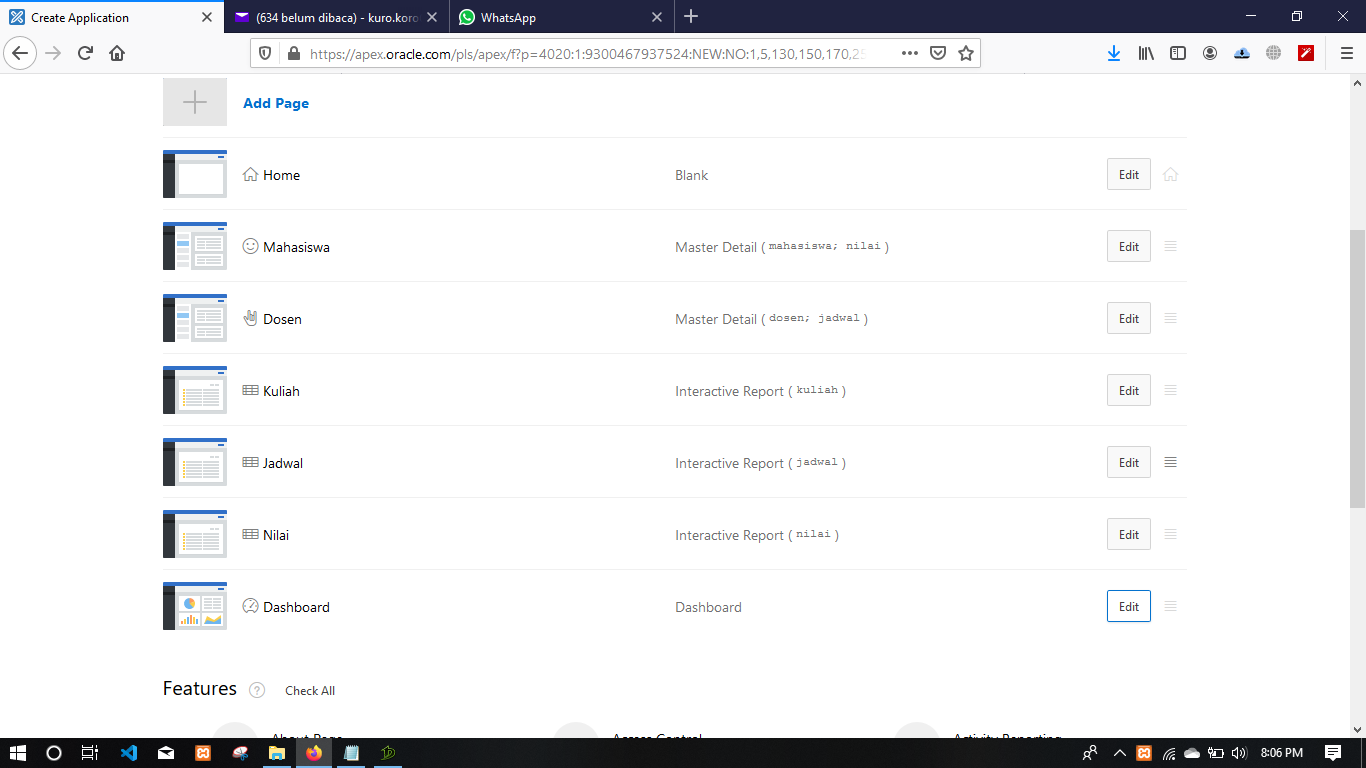
\includegraphics[scale=0.2]{figures/28.png}
    \end{center}   
    \end{figure}
    
\par
Tampilan Page yang sudah kita isi. Kemudian Klik Finish/Create 

\item[26]Kemudian RUN APPLICATION

\begin{figure}[!htbp]
    \begin{center}
    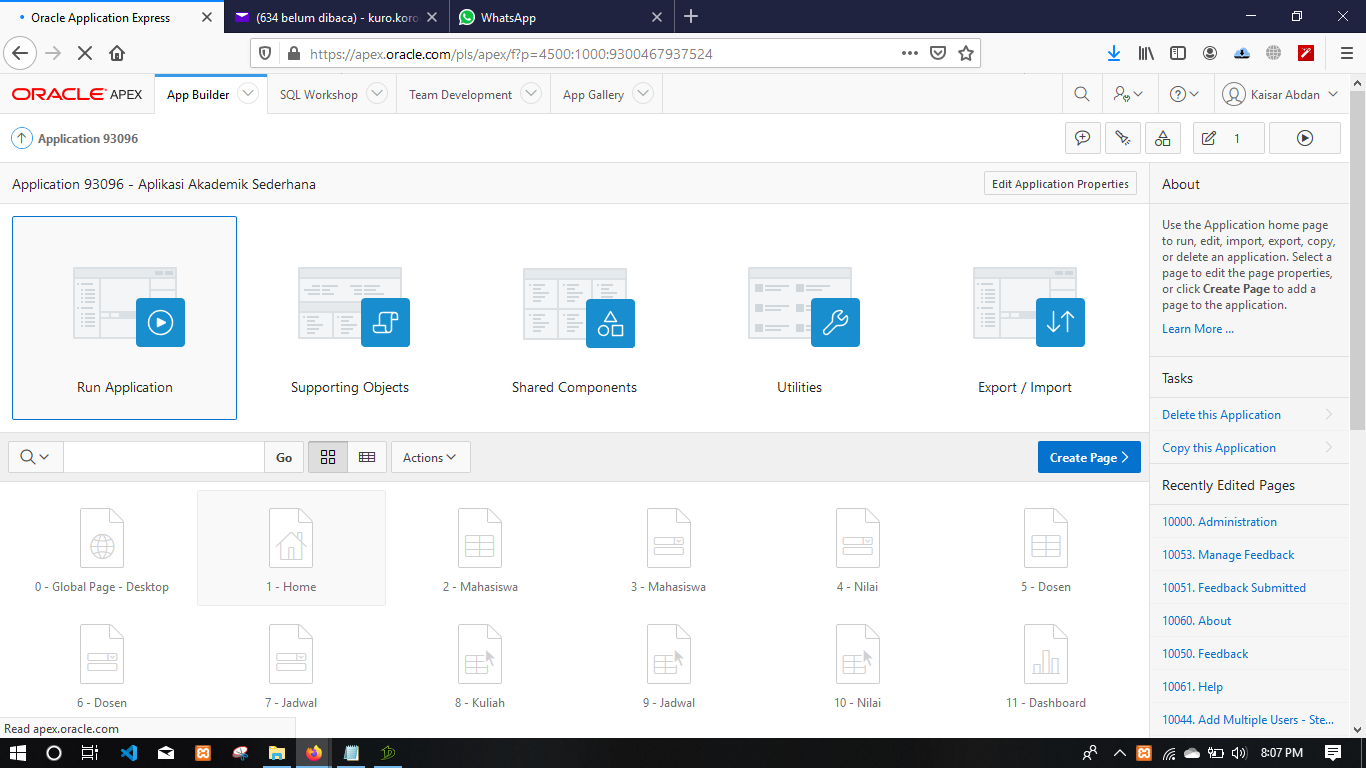
\includegraphics[scale=0.2]{figures/29.png}
    \end{center}   
    \end{figure}
    
\par
Ini Tampilan Saat kita akan Klik RUN APPLICATION.

\newpage
\item[27]Setelah Klik Run Application, Kita Harus Login Untuk Menjalankan Aplikasi yang sudah dibuat

\begin{figure}[!htbp]
    \begin{center}
    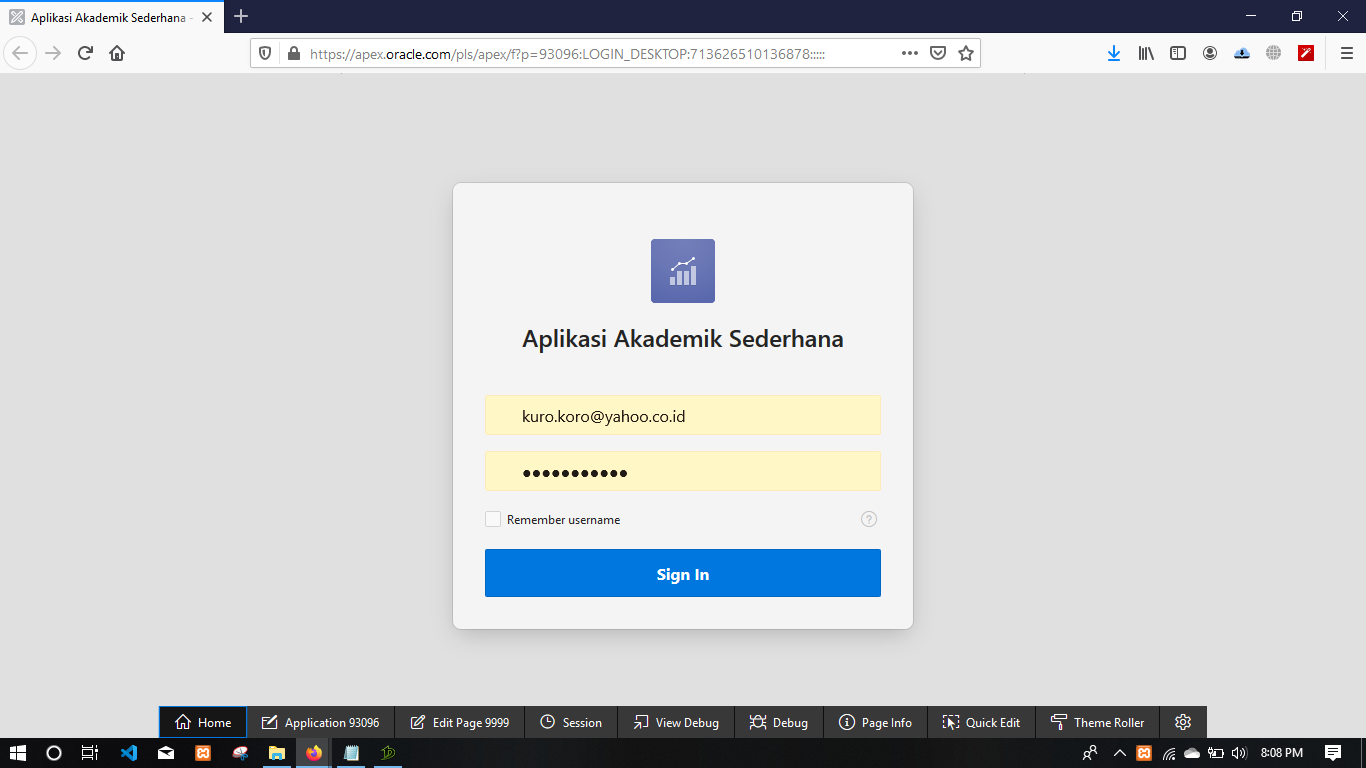
\includegraphics[scale=0.2]{figures/49.png}
    \end{center}   
    \end{figure}
    
\par
Disini kita Login Dengan Akun Kita Agar Aplikasi Dapat Dijalankan.

\item[28]Setelah Login, ini Tampilan Aplikasi yang sudah dibuatnya.

\begin{figure}[!htbp]
    \begin{center}
    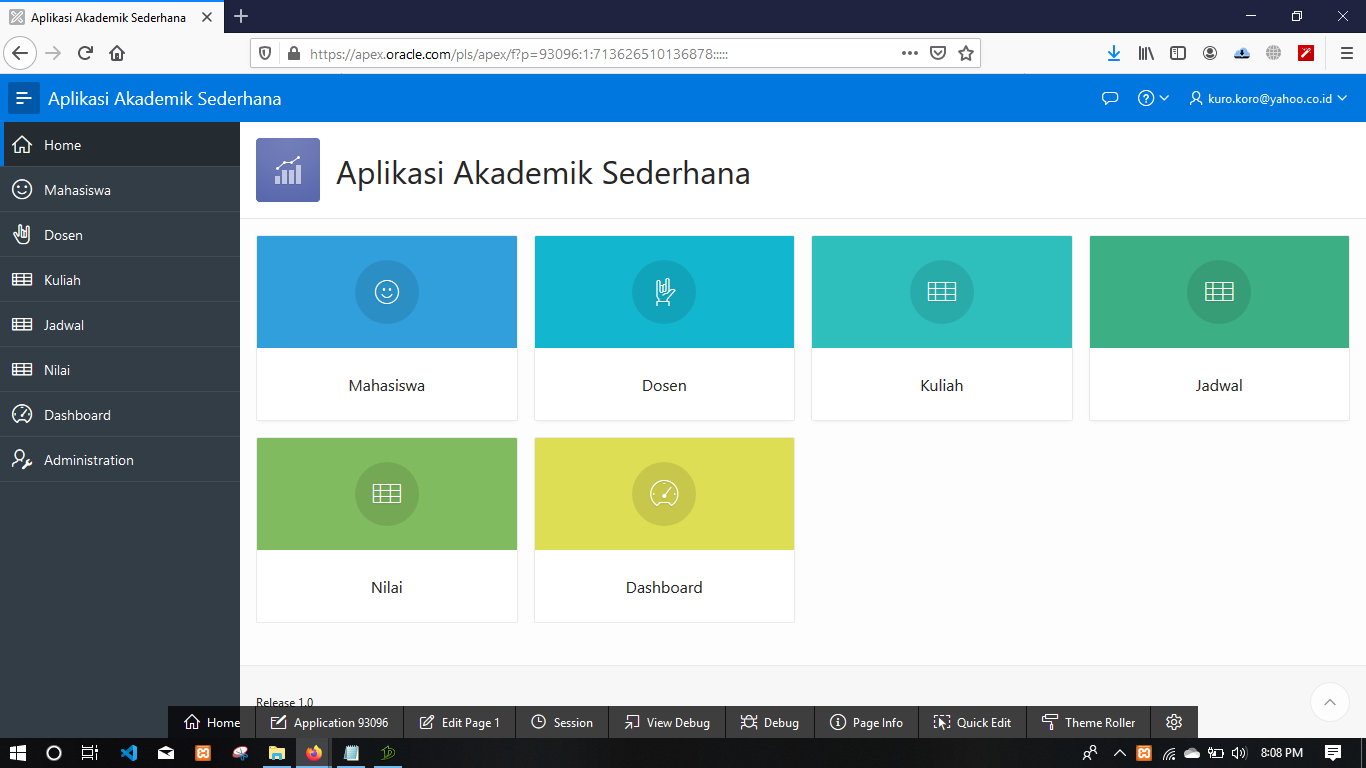
\includegraphics[scale=0.2]{figures/30.png}
    \end{center}   
    \end{figure}
    
\par
Selamat Aplikasi Anda Telah Dibuat, Anda dapat menjalankan APlikasinya.

https://apex.oracle.com/pls/apex/f?p=93096:1:730517775429531:::::
kuro.koro@yahoo.co.id
223790549Ka
    
\end{enumerate}


